% Generated from 10-世界模型、环境建模与可预测表征.md; edit the LaTeX source after migration.

\part*{第十部分 世界模型、环境建模与可预测表征}
\addcontentsline{toc}{part}{第十部分 世界模型、环境建模与可预测表征}
\markboth{第十部分 世界模型、环境建模与可预测表征}{第十部分 世界模型、环境建模与可预测表征}

在学习型机器人和多模态基础模型之间，世界模型路线扮演着一个非常微妙的角色。它既不像传统控制模型那样完全显式，也不像纯感知模型那样只负责当前观测解释，而是试图让系统形成一种能压缩环境、预测未来、支持规划的内部状态结构。也正因为这个位置特殊，世界模型在当前具身智能叙事中既被寄予厚望，也被广泛误读。

本部分的目标，不是把“世界模型”当作一个新口号，而是澄清三个问题：它到底在建模什么，它与控制模型、仿真器和 VLA 有什么区别，它在哪些地方真正有价值，又在哪些地方暂时还不应被高估。

从谱系上看，世界模型并不是今天才出现的概念。早期代表工作已经分别沿着“潜空间建模”“想象式展开”和“抽象表征预测”三条线推进：World Models 强调内部环境想象，Dreamer 把潜动态模型与策略学习更紧密地耦合，JEPA 则把重点从像素重建转向抽象表征预测。 相关代表性工作可参见 \href{https://arxiv.org/abs/1803.10122}{World Models：潜空间想象模型}、\href{https://arxiv.org/abs/1912.01603}{Dreamer：潜动态与策略耦合} 与 \href{https://arxiv.org/abs/2301.08243}{JEPA：联合嵌入预测架构}。这些工作共同说明，世界模型真正关心的不是“看起来像世界”，而是“是否保留了足以支持决策和规划的可预测结构”。

\chapter*{46. 世界模型的基本定义}
\addcontentsline{toc}{chapter}{46. 世界模型的基本定义}
\markboth{46. 世界模型的基本定义}{46. 世界模型的基本定义}

\section*{46.1 什么是“世界模型”}
\addcontentsline{toc}{section}{46.1 什么是“世界模型”}


这个定义里最关键的限定词其实是“对决策有用”。如果一个模型只能生成看起来合理的未来画面，却不能改变动作排序、风险筛选或训练数据价值评估，那么它更像生成器而不是机器人意义上的世界模型。相反，一个模型即便不产出漂亮视频，只要能稳定回答“哪一个候选动作更可能成功、哪一个更可能越界、哪一段 rollout 已经不可信”，它就更接近本报告讨论的具身世界模型。 在本报告语境里，世界模型可以先用一个朴素定义把握：它是机器人对“如果我这样动作，世界接下来大概率会怎样变化”的内部可计算近似。这个近似既可以在像素空间里预测未来，也可以在潜空间、语义空间或接触状态空间里预测未来。关键不在表示形式，而在它是否为后续规划、控制或数据生成提供了可用的因果近似。

一个最小抽象可以写成：

\begin{equation*}
\hat{s}_{t+1}, \hat{r}_t = f_\theta(s_t, a_t)
\end{equation*}

如果状态 \(s_t\) 不直接可得，则往往先引入编码器，把观测 \(o_t\) 映射为潜状态 \(z_t\)，再在潜状态中预测转移。更完整地写，世界模型通常不是一个单函数，而是一组职责明确的子模块：

\begingroup
\scriptsize
\begin{equation*}
z_t = e_\phi(o_t), \qquad
\hat{z}_{t+1} = f_\theta(z_t, a_t), \qquad
\hat{y}_t = h_\psi(z_t)
\end{equation*}
\endgroup

其中 \(e_\phi\) 是编码器，\(f_\theta\) 是潜动力学，\(h_\psi\) 则是任务头，用于预测奖励、风险、接触事件、终止条件或未来观测摘要。把这一分解写清楚非常重要，因为它解释了为什么“视频预测器”“潜空间动力学模型”和“带奖励头的规划模型”虽然都可能被叫作世界模型，但实际上服务的系统职责并不相同。若只有观测重建头而没有行动相关任务头，它更接近未来观测生成器；若能够稳定输出风险、回报或阶段转移，它才更接近规划可消费的内部世界近似。 这一定义之所以值得反复强调，是因为近两年“世界模型”一词被过度扩张，几乎任何能做未来建模、视频生成、隐状态更新或序列预测的系统都可能自称世界模型。但对机器人来说，真正有意义的判据始终是：它是否帮助系统减少真实试错、提高候选动作评估质量，或者增强对环境演化的结构化掌握。若做不到这些，只能说明模型具有某种预测能力，还不能说明它已经进入具身主链条。

对具身系统而言，世界模型最朴素的含义，是系统内部存在某种可预测环境和状态演化的模型，使它不仅知道“现在看到什么”，还能够在一定程度上回答“接下来可能发生什么”。这一定义比“能生成视频”更宽，也比“有隐藏状态”更严格，因为关键不在于压缩本身，而在于这种压缩是否支持未来预测和行动决策。

\section*{46.2 世界模型与控制模型、仿真器的区别}
\addcontentsline{toc}{section}{46.2 世界模型与控制模型、仿真器的区别}


世界模型、控制模型和仿真器看起来都在“预测未来”，但职责并不相同。控制模型更偏向低层局部动力学近似，常服务于 MPC、轨迹优化或解析控制器；仿真器则是更完整的环境生成与交互平台，需要负责物理、传感器、对象和任务脚本；世界模型通常处在二者之间，它不一定要求全物理保真，但要求对决策真正相关的未来结构做出紧凑、可学习、可调用的预测。

对学习者来说，可以先把三者粗略区分为：

\begin{enumerate}
\item \texttt{\detokenize{控制模型}}：偏低层、局部、服务控制器。
\item \texttt{\detokenize{仿真器}}：偏完整环境、可交互、服务训练与评测。
\item \texttt{\detokenize{世界模型}}：偏可学习内部预测器、服务规划与表征。
\end{enumerate}

控制模型通常更关注局部动力学和可控性；仿真器更关注完整环境重现；世界模型则往往更强调任务相关压缩和内部可预测性。三者当然可以重叠，但不能混同。一个模型可以生成看似逼真的未来视频，却未必适合控制；一个高保真仿真器可以很准确，却未必适合作为学习型内部状态表示。

从接口角度区分，控制模型最关心的是“给定当前状态与控制输入，短时局部动力学如何演化”；仿真器最关心的是“机器人与环境在更完整物理约束下如何共同演化”；世界模型则更像折中体，它不追求重建一切细节，而追求把对任务与规划最关键的未来结构压缩到一个可以快速推演的内部表示里。目标函数不同，评价标准也不同：控制模型看可辨识性与稳定性，仿真器看保真度与覆盖率，世界模型看规划可用性与分布外泛化下的结构是否仍可靠。 这一点在阅读文献时尤其重要。某些“视频世界模型”本质上更像生成式未来观察器，某些潜在动力学模型更像策略学习辅助器，某些数字孪生系统虽也预测未来，却主要服务于测试和验证而非内嵌闭环策略。若不先问清一个模型最终服务于控制、评测、数据生成还是内部规划，就很容易把不同问题设定下的结果误放到同一比较坐标系。

\section*{46.3 世界模型在机器人中的主要用途}
\addcontentsline{toc}{section}{46.3 世界模型在机器人中的主要用途}


这四种用途虽然常被放在一起讨论，但它们对模型质量的要求并不相同。若只作为训练期辅助环境，模型可以容忍更强的近似误差，只要它能提供有用梯度或额外样本；若直接参与在线规划，误差容忍度就会急剧收紧，因为错误会立即转化为错误动作评估。若作为失败恢复分析工具，模型则需要对异常后果和可回退分支更敏感，而不一定追求逼真重建。因此，阅读相关论文时，先识别“世界模型到底打算被用在哪个环节”，几乎是理解其价值的前提。

主要用途至少包括：

\begin{enumerate}
\item 作为策略学习的辅助内部环境。
\item 作为规划 rollout 的未来近似器。
\item 作为观测压缩与任务相关状态表示。
\item 作为数据增广或失败恢复分析工具。
\end{enumerate}

如果再往系统职责上细分，可以把它们理解为四种不同的消费方式：训练期消费、规划期消费、诊断期消费和记忆期消费。训练期消费更看重样本效率和表征质量，规划期消费更看重候选动作排序是否稳定，诊断期消费更看重失败后果与风险解释，记忆期消费则更看重长期状态压缩和任务阶段跟踪。这个区分有助于避免把所有“能预测未来”的模型都用同一把尺子评价。

更严格地说，机器人系统真正消费的并不是“未来图像”本身，而是某种可被下游模块读取的未来摘要。若把世界模型的输出统一写成

\begingroup
\scriptsize
\begin{equation*}
\hat{u}_{t:t+H} =
\left(
\hat{z}_{t:t+H},
\hat{r}_{t:t+H},
\hat{c}_{t:t+H},
\hat{m}_{t:t+H}
\right)
\end{equation*}
\endgroup

其中 \(\hat{z}\) 表示未来潜状态，\(\hat{r}\) 表示任务收益或进展，\(\hat{c}\) 表示约束代价或风险，\(\hat{m}\) 表示阶段标记、对象关系或可解释事件，那么四类用途的区别，本质上就在于谁来消费这些字段、哪个字段最重要、以及允许多大误差。训练期辅助环境最关心 \(\hat{z}\) 是否保留可学习结构；规划期最关心 \(\hat{r}\) 与 \(\hat{c}\) 的排序稳定性；诊断期更关心 \(\hat{m}\) 是否能把失败链条显式化；记忆期则更关心 \(\hat{z}\) 与 \(\hat{m}\) 是否足以支持长时程状态压缩。

这也是为什么“看起来同样在做世界模型”的工作，系统地位会非常不同。以 \href{https://arxiv.org/abs/2506.09985}{V-JEPA 2} 为例，其机器人分支 \texttt{\detokenize{V-JEPA 2-AC}} 不是把模型直接塞进高速控制回路，而是先利用大规模视频预训练形成动作条件世界模型，再用较少机器人视频做后训练，用于图像目标条件下的规划；这说明世界模型在当前更可信的职责之一，是把大规模表征先验转译成较低频的规划与排序能力。另一类工作如 \href{https://arxiv.org/abs/2505.19017}{WorldEval} 则进一步说明，世界模型甚至可以主要服务于“策略评估代理”而非“策略执行器”：其目标不是替机器人下动作，而是在线给不同策略和 checkpoint 做排序、筛除明显危险动作。这类工作特别值得注意，因为它把世界模型的使用位置从“控制之前”扩展到了“研发评估流程内部”。

因此，本章更倾向于把世界模型理解为一种“中间职责放大器”。它最有价值的时候，并不是自称统一了一切，而是非常清楚地声明：自己到底在为哪一个消费环节降低试错成本。只要这个位置说不清，所谓“世界模型很强”就很容易滑回一种抽象宣传；反过来，只要消费接口说清楚，即便模型不生成华丽视频，它也可能是系统里非常高杠杆的一层。

\chapter*{47. 动力学建模与潜空间预测}
\addcontentsline{toc}{chapter}{47. 动力学建模与潜空间预测}
\markboth{47. 动力学建模与潜空间预测}{47. 动力学建模与潜空间预测}

\section*{47.1 观测空间与潜空间}
\addcontentsline{toc}{section}{47.1 观测空间与潜空间}


因此，潜空间设计最需要追问的不是压缩率，而是“保留了哪些任务相关不变量”。对机器人来说，这些不变量往往不是纹理，而是对象身份、相对位姿、接触阶段、可达性关系、风险趋势和动作后果类别。潜变量若无法携带这些量，就算重建得再好，也很难服务规划；潜变量若只对当前任务过拟合，又会损害跨场景复用。这种张力解释了为什么后文很多路线会围绕对象中心潜变量、预测状态表征和任务条件潜变量展开分化。 观测空间与潜空间的差别，决定了模型是在“直接看原始世界”，还是先“压缩出一个更适合预测与决策的内部世界”。观测空间里的变量往往是高维、冗余、含噪的，例如图像、点云和多传感器原始流；潜空间则是编码器学习出来的低维内部状态，目标是保留与控制相关的信息，同时丢弃大量无关细节。

一个最小映射关系可以写成：

\begingroup
\footnotesize
\begin{equation*}
z_t = e_\theta(o_t), \qquad \hat{z}_{t+1} = f_\phi(z_t, a_t)
\end{equation*}
\endgroup

这里最重要的不是“压缩得小”，而是“压缩后是否仍保留可达性、接触、对象关系和任务阶段等对决策重要的结构”。

在高维视觉和多模态观测下，直接在原始空间预测未来往往既昂贵又脆弱，因此世界模型常常先把观测映射到潜空间 \(z_t\)，再在潜空间中建模时间演化：

\begingroup
\footnotesize
\begin{equation*}
z_t = e(o_t), \qquad z_{t+1} \sim p_{\theta}(z_{t+1}\mid z_t, a_t)
\end{equation*}
\endgroup

这个结构的意义，在于它试图把“什么对未来最关键”压缩进内部状态，而不要求像素级重建一切细节。

\section*{47.2 一步预测、多步预测与 rollout}
\addcontentsline{toc}{section}{47.2 一步预测、多步预测与 rollout}


一步预测关注“下一步会怎样”，多步预测与 rollout 关注“如果我连续做一串动作，未来一段时间会怎样演化”。前者通常更容易训练，因为误差只跨一个时间步；后者更贴近规划需求，因为真实机器人决策往往关心一整段动作后果。

其最小 rollout 过程可以写成：

\begin{lstlisting}[language=python]
z0 = encoder(obs)
for seq in candidate_action_sequences:
    z = z0
    score = 0.0
    for action in seq:
        z = dynamics(z, action)
        score += reward_head(z) - lambda_risk * risk_head(z)
    rank(seq, score)
\end{lstlisting}

也正因此，很多世界模型论文虽然首先报告一步预测误差，但真正决定系统能否用于规划的，往往是多步 rollout 是否稳定。这个代码片段明确揭示了一件常被忽略的事实：rollout 不是为了“把未来完整演给人看”，而是为了给一组候选动作序列提供可比较的内部评分。 这里还隐含着一个常被忽略的接口问题：rollout 不是为了把未来完整演一遍，而是为了给某个决策变量提供比较依据。也就是说，多步预测是否有价值，取决于它是否改善了动作排序、风险筛选或计划修复，而不取决于它是否生成了“更长更像真的未来”。这一区分很重要，因为许多生成式模型在视觉上极具说服力，却未必在决策排序上比简单短视估计更可靠。

一步预测往往较容易，但世界模型真正有吸引力的地方在于多步 rollout：系统可以在不真实执行的情况下，对未来若干步结果做内部想象。这一点对高代价机器人任务尤其诱人，因为真实试错很慢，内部 rollout 看似提供了一条更廉价的规划路径。

若在潜空间中做 \(H\) 步 rollout，则可写为：

\begingroup
\footnotesize
\begin{equation*}
\hat{z}_{t+k+1} = f_\theta(\hat{z}_{t+k}, a_{t+k}), \qquad k=0,\dots,H-1
\end{equation*}
\endgroup

并通过某个任务头 \(r_\phi(\hat{z}_{t+k})\) 评估回报、风险或任务进展。

若再把动作序列排序目标显式写出来，则更接近规划时真正优化的量：

\begingroup
\scriptsize
\begin{equation*}
J(a_{t:t+H-1}) =
\sum_{k=0}^{H-1} \gamma^k \hat{r}_{t+k}
- \lambda \sum_{k=0}^{H-1} \hat{c}_{t+k}
\end{equation*}
\endgroup

其中 \(\hat{r}_{t+k}\) 可以表示任务收益或进展，\(\hat{c}_{t+k}\) 可以表示碰撞、越界、失稳或失败风险。这个式子提醒我们，世界模型的真正价值不在于“预测得多丰富”，而在于它是否让 \(J(\cdot)\) 的排序结果比没有模型时更可靠。

这段公式真正想表达的，不是“世界模型会自己产生价值”，而是它只有在后面接上决策评价头时才有系统意义。也就是说，rollout 的目的并不是做未来电影，而是比较候选动作的后果差异。若模型无法稳定区分“这个动作会撞上障碍”和“那个动作更可能顺利接触目标”，那么即便它能生成长而连贯的未来片段，也未必值得在机器人系统中承担核心职责。

\section*{47.3 长时程误差累积问题}
\addcontentsline{toc}{section}{47.3 长时程误差累积问题}


但多步 rollout 的根本问题同样明显：每一步小误差都会继续传递，最终使远期预测迅速失真。也就是说，世界模型越被用作长时程推演工具，就越必须面对累积误差和分布外偏移。

这里最容易产生的误解，是把“预测图像越清晰”与“决策支持越可靠”等同起来。对机器人而言，远期 rollout 的真正价值并不在于每一帧都像真实视频，而在于它能否保持关键决策顺序的稳定性，例如哪条路径更可能避开障碍、哪个接触策略更可能导致滑脱、哪个动作序列更容易把系统带入不可恢复状态。换言之，长时程预测的有效性首先体现在相对排序是否正确，而不是像素级还原是否精细。

工程上应对误差累积的思路，通常不是盲目把 rollout 拉得更长，而是限制模型承担的时间尺度，并让其与闭环校正机制耦合。例如只在若干关键决策节点做有限步 lookahead、在每次新观测到来后重置隐状态、或把世界模型用于候选动作筛选而不是端到端控制。这样做等于承认模型的远期可信度有限，但仍尽量保留其在局部后果评估上的系统价值。

因此，在阅读相关论文或产品宣称时，一个更稳健的判断问题是：该世界模型究竟被部署在什么时间尺度上，它的误差会如何被观测更新、控制反馈或安全约束吸收？若这些问题没有被回答，那么“支持长时程推演”的表述通常更接近一种研究愿景，而不是已经可交付的系统能力。

在机器人里，这个问题比纯视觉预测更严重，因为系统不会只“看着模型出错”，而会真的按照错误预测去行动。短期偏差可能只影响下一帧重建，但闭环执行会把这种偏差进一步放大，并把机器人推向训练中更少见的新状态分布，随后模型又在这个更偏的分布上继续预测，于是形成典型的“闭环累积误差”。 这也是为什么真实系统中的世界模型通常不会被当作“远期全知模拟器”，而更像带不确定性边界的有限视距评估器。工程上常见的缓解策略包括短视重规划、风险头估计、模型集成、保守候选筛选与不确定性触发回退，而不是盲目拉长 rollout 长度。

若把单步预测误差记为 \(\epsilon_t\)，那么多步 rollout 的有效误差通常会近似呈累加甚至放大趋势：

\begingroup
\footnotesize
\begin{equation*}
\|\hat{z}_{t+H} - z_{t+H}\| \lesssim \sum_{k=0}^{H-1} L^{H-1-k}\epsilon_{t+k}
\end{equation*}
\endgroup

这里的 \(L\) 可以被粗略理解为动力学映射对误差的放大系数。即使单步误差不大，只要系统对偏差敏感、或 rollout 足够长，整体误差就会迅速劣化。这也是为什么很多机器人世界模型最终更适合承担短视重排序、局部风险筛选或训练期辅助角色，而不是直接接管很长时域的在线控制。

\begingroup
\footnotesize
\begin{equation*}
\|\hat{z}_{t+H} - z_{t+H}\| \not\approx \epsilon_t,
\qquad
\text{often grows with } H
\end{equation*}
\endgroup

这不是形式化上必须线性增长，而是提醒我们：哪怕单步模型“还不错”，也不能直接推断长时程规划就可靠。对机器人而言，关键不是把 rollout 做得尽可能长，而是找到在当前误差水平下仍具决策价值的预测视距。

很多系统因此会显式估计一个“有效预测视距”：

\begingroup
\footnotesize
\begin{equation*}
H_{\mathrm{eff}} = \max \left\{ H \;|\; u(\hat{z}_{t+H}) \le \tau \right\}
\end{equation*}
\endgroup

其中 \(u(\hat{z}_{t+H})\) 表示随 rollout 长度增长而上升的不确定性或置信衰减，\(\tau\) 是系统可接受阈值。这个定义非常贴近工程实践，因为它把“模型到底能想多远”从抽象宣传口号改写成了一个可被在线监测的系统变量。真正成熟的机器人系统通常不会无条件相信长 rollout，而会在 \(H > H_{\mathrm{eff}}\) 时主动缩短规划视距、请求新观测、触发重规划或回退到更保守控制器。

\section*{47.4 隐状态是否真的学到了“物理”}
\addcontentsline{toc}{section}{47.4 隐状态是否真的学到了“物理”}


更严格地说，我们更关心的是“是否学到了对行动后果稳定有用的物理”，而不是“是否长得像物理”。一个潜状态不需要显式长成质量、摩擦系数、法向力这样的可解释变量才可能有用；但如果它在动作改变、接触发生、外界扰动出现时无法保持结构稳定，那么它再难解释也很难用于可靠控制。因此，对具身系统而言，物理性的判据最终是干预下的预测稳定性与任务可用性，而不是视觉可解释性本身。

这是世界模型争论中最关键的问题之一。一个潜状态可能非常有利于短期预测，却并不等于它编码了可解释的物理变量；它也可能只是“对当前训练分布足够有效”的压缩表示。因此，世界模型是否真的学到了与对象、接触、动力学因果机制相关的结构，必须依靠泛化表现、规划效果和干预鲁棒性来判断，而不能只凭重建或预测视觉效果下结论。

更可操作的判断方式是看这种隐状态在动作干预下是否保持结构稳定。例如，当接近路径改变、抓取方向改变、接触是否发生发生变化时，模型内部状态是否还能维持对后续结果的可区分性。若内部状态只在被动视频延续条件下稳定，而一旦动作改变就迅速崩塌，那么它更可能是视觉统计压缩，而不是行动相关结构表示。

这也意味着，对世界模型的评价不能只停留在“预测误差小不小”，而要追问“在动作改变时内部结构是否仍然有用”。对具身系统来说，真正稀缺的是行动相关稳定性，而不是被动观察下的压缩优雅性。

\chapter*{48. 视频预测与生成式环境建模}
\addcontentsline{toc}{chapter}{48. 视频预测与生成式环境建模}
\markboth{48. 视频预测与生成式环境建模}{48. 视频预测与生成式环境建模}

\section*{48.1 视频生成作为世界建模的路径}
\addcontentsline{toc}{section}{48.1 视频生成作为世界建模的路径}


把视频生成视为世界建模的一条路径，吸引力在于它提供了一个直观目标：让模型预测“下一步世界会长成什么样”。若模型能在长时间尺度上生成与动作条件一致的未来观测，人们自然会期待它内部已经学习到足够有用的动力学、因果与可供性结构。

但机器人场景中最大的风险是把“视觉上逼真的未来帧”误判成“对控制有用的世界模型”。对动作决策真正关键的，未必是像素级纹理细节，而是接触前后的状态转移、可达约束、碰撞边界和任务结果变量。一个模型即使能生成很像真的视频，也可能没有把最关键的动作可执行信息稳定编码出来。

因此，视频生成路线更适合作为世界建模的一个可观测代理，而不是充分定义。对机器人而言，最重要的追问永远是：这个生成模型能否支持规划、反事实评估、异常预判或数据合成，而不是它生成的视频是否“像电影”。如果不能反哺动作闭环，那么它更像通用视频建模，而不是真正服务具身系统的世界模型。

视频生成路线吸引人的地方，在于它看起来提供了一种统一表述环境变化的方法：只要系统能预测未来帧，就似乎同时掌握了对象运动、遮挡变化、交互结果和任务后果。这种统一性对研究者极具诱惑，因为它让世界建模问题被重新包装成了大规模视觉生成问题。

但从机器人角度看，视频生成真正有价值的前提，是它生成的变化必须与动作条件、接触约束和因果后果有稳定对应关系。否则，模型学到的更可能是“视觉上像未来的画面”，而不是“行动后真的会发生的未来”。因此，视频生成是世界建模的一条路径，但不是世界建模本身。 这条路线的真正吸引力，在于它天然承接了互联网规模视频预训练与生成模型基础设施，使世界建模不再完全依赖机器人专属数据。也就是说，它为“先在开放世界学未来变化结构，再向具身任务迁移”提供了看似可行的桥梁。问题在于，这座桥梁往往更擅长迁移视觉统计规律，而不是迁移可执行交互规律，因此必须特别警惕“开放世界未来感”与“机器人可执行未来”之间的错位。

随着生成模型能力上升，视频预测开始被视为世界建模的一条自然路径。原因很直观：如果模型能根据当前观测和动作生成未来视频，那么它似乎就“知道世界会怎样变化”。

\section*{48.2 diffusion/video model 的优势与代价}
\addcontentsline{toc}{section}{48.2 diffusion/video model 的优势与代价}


生成式视频模型的优势，在于它们能表达更丰富、更高维、更不确定的未来分布；代价则在于训练昂贵、推理昂贵，而且生成逼真并不自动意味着预测对控制有用。对机器人来说，最关键的问题不是生成视频看起来是否自然，而是这些未来是否保留了任务相关的物理可执行结构。

扩散与视频生成路线之所以极具吸引力，是因为它们似乎天然拥有开放世界建模能力。面对复杂背景、多对象交互和长尾视觉变化，它们确实往往比简单重建式 latent model 更有表达力。但机器人规划并不消费“像真度”本身，而消费与动作后果相关的结构变量，例如可抓取性、碰撞风险、接触后稳定性与局部几何一致性。只要这些变量没有被稳定编码进去，再漂亮的未来视频也可能只是视觉幻觉。 若把这一路线写成抽象生成形式，可以表示为：

\begin{equation*}
x_{t+1:t+H} \sim G_\theta(x_{\le t}, a_{t:t+H-1}, \xi)
\end{equation*}

其中 \(x\) 表示视频观测，\(a_{t:t+H-1}\) 是动作条件，\(\xi\) 则表示生成过程中的随机变量或噪声。这个写法说明，扩散/视频模型天然擅长描述“多种可能未来”，但并不保证这些未来都对控制有用。机器人系统若要消费它，往往还得在生成结果之上增加对象级、接触级或风险级任务头，把海量像素未来重新压缩回可执行结构。

因此，更严格的评价问题是：这种生成模型能否被压缩成低时延、可条件控制、可被策略反复查询的规划接口。如果不能，它更可能是一种研究资产、数据生成器或分析工具，而不是立即可落地的闭环核心。

从系统工程角度看，它们的主要代价至少包括三类：第一是训练与推理成本高，难以进入高频在线环；第二是预测对象往往过于“视觉化”，与控制变量之间还隔着一层接口翻译；第三是评价口径容易被视觉说服力误导。也就是说，视频生成模型最容易赢得演示效果，却最需要在规划价值和控制可消费性上被额外严格审查。

更进一步说，这类模型在机器人里通常只有三种较稳妥的职责位置。第一，作为离线分析器，用于检查策略在不同动作条件下可能遇到的未来变化；第二，作为数据生成器，用于扩充某些长尾视觉场景；第三，作为上层候选过滤器的一部分，在较低频率上为若干候选计划提供粗粒度未来比较。凡是想让它直接进入高频闭环、细粒度接触控制或严格安全约束回路的方案，都必须比普通视频模型接受更高强度的审查。

这一定义对后续阅读很多“world model + video”路线特别重要。只要没有回答它如何进入规划接口、是否满足时延预算、以及是否优于更简单的结构化预测，那么它就仍更像研究资产，而不是系统核心部件。

\section*{48.3 生成逼真不等于物理正确}
\addcontentsline{toc}{section}{48.3 生成逼真不等于物理正确}


生成逼真不等于物理正确，这是世界模型研究里最容易被忽略的基本事实。一个视频可以在视觉上非常连贯、纹理细节丰富、对象外观自然，却仍然违反接触约束、质量守恒、刚体运动规律或任务逻辑顺序。对旁观者来说它“像真的”，对机器人来说它却可能没有足够的决策价值。

也正因为如此，世界模型不能只按人类主观观感来评价。真正关键的问题是：它的预测是否保留了对动作后果最关键的可验证结构，是否能支撑规划、筛选候选动作和评估风险，而不是仅仅生成一段漂亮的未来片段。 对于操作任务，这种错位尤其严重，因为很多成败恰恰由肉眼不显著的局部物理决定。例如，夹爪与物体边缘的相对姿态差几毫米、摩擦方向略有变化、插孔对位误差在视觉上几乎看不出，但它们足以让一个任务从成功变成卡住或滑脱。视频生成模型若只在宏观视觉连贯性上成功，却不能稳定表达这些微观结构，对机器人规划的帮助就会十分有限。

这是世界模型讨论中最容易被忽视的一点。一个模型可以生成肉眼看来“合理”的对象运动，却在接触细节、动力学约束、可抓取性和时间同步上全部失真。于是，生成美观的未来与提供可用于控制的未来，常常是两件不同的事。

对学习者而言，一个很实用的区分方法是：先问这个模型是否在“控制相关变量”上正确。所谓控制相关变量，可能是接触是否发生、可达区域是否改变、对象是否被稳定抓住、障碍物是否进入危险区，而不一定是整段视频看起来多自然。只有把评价口径从“像不像”改成“能不能支持动作判断”，世界模型章节才不会退化为生成模型章节的附庸。

\section*{48.4 为什么视频预测在开放世界里诱人}
\addcontentsline{toc}{section}{48.4 为什么视频预测在开放世界里诱人}


视频预测在开放世界里之所以诱人，是因为它似乎绕开了显式状态设计的痛苦。面对开放环境、长尾物体和复杂场景时，研究者很难手工定义一套完备状态变量；而视频作为统一观测表述，看起来天然能覆盖所有变化。这使得它在开放世界中具备很强的“接口统一”吸引力。

不过，这种诱惑也伴随风险。视频预测越通用，越容易把真正重要的可执行结构淹没在大量视觉细节中。对于机器人而言，开放世界不只需要“预测更多”，还需要在预测中保留那些与行动选择直接相关的因果骨架。

尽管问题很多，视频预测仍然有吸引力，因为它天然适合容纳开放环境中的对象变化、背景变化和多种可能未来。在互联网时代训练出来的大规模生成模型，也让“未来想象”这件事在技术上更可行。但对具身系统来说，这条路线能否成立，最终仍要看它是否能被压缩成规划可用、时延可接受、可与动作接口闭合的内部结构。

换句话说，视频预测真正迷人的地方，在于它提供了一种看似统一的世界接口；而它真正危险的地方，也在于这种统一过于诱人，容易让人忽视“统一到了视觉层，不等于统一到了行动层”。这也是本章坚持把视频生成和抽象预测分开讨论的原因。

近两年这条路线重新升温，一个重要原因正是大规模视频先验的可用性显著提升。\href{https://arxiv.org/abs/2506.09985}{V-JEPA 2} 展示了“先在超过一百万小时互联网视频上预训练，再用少量机器人轨迹后训练”的路线，这类工作极具吸引力，因为它似乎提供了一条把开放世界视频知识迁移到机器人规划的捷径。对研究者而言，这种路线最诱人的不是“视频更逼真”，而是“也许不必先把对象、接触、动力学全部手工结构化，模型就能自己形成足够有用的未来表征”。

但这条路线的主要反证也越来越清楚。当前很多视频世界模型本质上仍工作在二维序列上，因此对机器人最关键的三维几何、跨视角一致性和物理约束保留不足。\href{https://arxiv.org/abs/2606.18375}{PAIWorld：面向机械臂操作的三维一致性世界基础模型} 直接指出，现有多视角世界模型若只是拼接不同视角的 token，而没有显式几何先验和视角间通信机制，就会出现跨视角对象漂移、深度不一致和纹理错位；\href{https://arxiv.org/abs/2607.01166}{Structured 4D Latent Predictive Model：面向机器人规划的四维结构化潜变量预测模型} 则进一步强调，单纯二维视频序列缺乏精确空间推理所需的三维几何理解。这些工作并不是在否定视频路线，而是在提醒我们：只要下游任务需要精确接触、相对位姿和多视角闭环，纯视频 token 统一接口很容易在最关键的地方失真。

因此，对机器人而言，视频预测是否“足够好”的判据，不应只看视觉连贯性，而应看它是否保留了最小行动结构集：

\begingroup
\scriptsize
\begin{equation*}
\mathcal{S}_{\text{act}} =
\{
\text{relative pose},
\text{contact onset},
\text{occlusion cause},
\text{reachability change}
\}
\end{equation*}
\endgroup

若模型生成的未来没有稳定保留这组结构，那么它再开放、再通用，也更接近“世界观测生成器”而不是“行动相关世界模型”。这也是为什么视频世界模型在具身系统里更适合作为上游候选能力，而不是自动享有最终控制资格。

\chapter*{49. JEPA 与抽象预测路线}
\addcontentsline{toc}{chapter}{49. JEPA 与抽象预测路线}
\markboth{49. JEPA 与抽象预测路线}{49. JEPA 与抽象预测路线}

\section*{49.1 不重构像素而预测语义}
\addcontentsline{toc}{section}{49.1 不重构像素而预测语义}


这一类方法的核心出发点，是承认“像素级重建并不一定等于控制相关预测”。如果任务真正关心的是对象是否可达、是否被遮挡、是否发生接触、是否进入危险区域，那么直接要求模型重建每一个像素，可能把大量容量浪费在与决策无关的细枝末节上。

因此，JEPA 一类方法更强调预测抽象表征而非原始像素，即：

\begin{equation*}
\hat{z}_{t+k} = f_\theta(z_t, a_{t:t+k-1})
\end{equation*}

其中 \(z\) 表示抽象语义状态。若进一步写成更接近 JEPA 思想的上下文 - 目标形式，则可以表示为：

\begingroup
\scriptsize
\begin{equation*}
z_t^{ctx} = e_\phi(c_t), \qquad
z_{t+k}^{tar} = e_\phi(u_{t+k}), \qquad
L_{\mathrm{JEPA}} = \left\| p_\theta(z_t^{ctx}, a_{t:t+k-1}) - z_{t+k}^{tar} \right\|_2^2
\end{equation*}
\endgroup

这里 \(c_t\) 表示上下文视图或历史片段，\(u_{t+k}\) 表示未来目标视图或未来抽象状态，\(p_\theta\) 则是预测器。这个目标的关键不是“把未来像素重新画出来”，而是让模型在抽象空间里学会“从当前上下文和动作条件推断未来应当保持哪些结构”。对机器人而言，这种目标更贴近世界模型应承担的职责，因为很多决策真正依赖的是对象关系、任务阶段和接触后果，而不是背景纹理是否逐像素一致。

对机器人而言，这一路线的吸引力在于它可能更容易保留任务结构，而不是被纹理细节牵着走。 如果把这一路线放回具身系统接口中理解，其价值就在于主动声明“预测目标应该为决策服务，而不是为视觉还原服务”。也就是说，模型可以不去还原每一个纹理细节，而把容量优先分配给对象关系、状态变化、动作后果与任务阶段这样的高价值变量。这种取舍与机器人系统的需求是更一致的，因为执行系统最终消费的是可执行结构，而不是美观视频。

JEPA 路线的重要性，在于它试图绕开像素级重建这一高成本目标，转而预测更抽象的表征结构。\href{https://arxiv.org/abs/2301.08243}{JEPA} 这对于机器人尤其有吸引力，因为机器人真正需要的往往不是像素复刻，而是对行动相关语义与结构的稳定预测。

\section*{49.2 抽象预测与因果结构}
\addcontentsline{toc}{section}{49.2 抽象预测与因果结构}


抽象预测路线强调，不必强迫模型逐像素重建未来，而可以只预测对决策真正重要的潜变量、关系结构或任务相关状态。这一思路的核心不是偷懒，而是承认控制问题所需的信息远少于完整感官重建。对于机器人来说，未来的接触状态、物体关系、可通行拓扑或阶段性子目标，往往比精确纹理更重要。

从概念上看，抽象预测更接近学习

\begin{equation*}
z_{t+1} = f_\theta(z_t, a_t)
\end{equation*}

而不是直接学习像素空间里的 \(o_{t+1}\)。若 \(z_t\) 真的保留了因果上关键的状态变量，那么模型就更可能在分布变化下维持有效预测，因为它抓住的是结构而不是表象。

但“抽象”二字也最容易被滥用。若潜变量只是压缩后的表面统计量，而没有与动作后果、对象关系或约束结构建立稳定对应，那么所谓抽象预测也可能只是另一种不透明压缩。因此，本章讨论因果结构时必须保持克制：重点不在宣称模型“学到了因果”，而在检验它是否学到了对干预、规划和异常恢复真正有用的稳定结构。

如果世界模型只学习表面共现模式，它在环境变化和分布外场景中往往非常脆弱。抽象预测路线的潜台词是：系统应尽量学习那些更接近对象、关系、交互机制和任务结构的内部对象，而不是沉迷于重建所有可见细节。

但“抽象”并不自动等于“因果”。一个 latent state 也可能只是更紧凑地压缩统计相关性，而没有真正分离出稳定机制变量。对具身系统而言，真正重要的是这些内部变量能否支持干预式推理：当动作改变、接触方式改变或环境配置改变时，模型是否能给出结构上合理的未来分支，而不是仅仅延续训练集中最常见的视觉惯性。 因此，世界模型若想从“预测器”进化为“规划器”，最终必须在某种程度上面向干预、反事实与任务相关因果结构。哪怕做不到严格可解释，它也至少应在动作改变后表现出稳定的结构响应，而不仅在被动观察条件下维持高分。

对机器人来说，这个“因果结构”最务实的检验方式往往不是哲学意义上的因果发现，而是工程意义上的干预一致性：同一对象在不同接近方向下是否呈现不同但合理的接触后果，同一技能在不同环境约束下是否能预测不同失败模式。只要模型能在这些关键干预维度上给出稳定差异，它就比只会延续视频表面的模型更接近真正可用的世界模型。

\section*{49.3 JEPA 路线对机器人世界建模的启发}
\addcontentsline{toc}{section}{49.3 JEPA 路线对机器人世界建模的启发}


JEPA 路线的重要启发，在于它试图把预测目标从低层细节重建转向高层一致性预测。对机器人来说，这很有吸引力，因为具身系统往往不需要准确预测每个像素，而更需要预测“在当前动作与上下文下，哪些高层结构将保持，哪些会变化”。这种训练目标有潜力减少模型把容量浪费在纹理与背景上，而把更多表示能力留给对象关系、动态结构与任务相关状态。

如果把 JEPA 式思想迁移到机器人，可以把它理解为：给定历史观测和动作条件，预测未来表征空间中那些稳定但又对任务有区分度的部分。这类目标尤其适合与时序一致性、多视角对齐、动作条件预测和本体状态联合建模结合，形成更贴近控制需求的世界表示。

但它的局限也必须说清楚。JEPA 风格目标并不会自动告诉我们“哪些抽象量最适合机器人控制”，更不会自动解决接触、稀有异常或跨本体映射问题。它提供的是一个值得重视的表示学习方向，而不是直接可部署的世界模型答案。真正的价值在于：它帮助我们重新界定“机器人到底需要预测什么”，而不只是继续在像素重建上堆资源。

JEPA 路线的重要启发，在于它提醒机器人研究者：未必要把所有未来都重构成像素，才能获得有用的预测能力。若系统能在抽象空间中预测那些真正决定后续决策的结构变量，例如对象关系、可达状态、任务阶段和潜在风险，那么它也许能用更低成本获得更稳定的长时程表征。

这一路线对机器人尤其有意义，因为真实控制常常并不需要照片级未来，而需要“什么东西会变、什么约束还成立、什么动作更可能成功”这样的结构信息。JEPA 类方法因此更接近把世界模型做成决策基础设施，而不是做成视觉特效引擎。 这也提示我们，未来很多真正有工程价值的世界模型可能既不像纯视频生成器，也不像传统显式动力学模型，而更像“任务结构优先的预测表征器”。它们会优先保留接触前后状态切换、对象可达性变化、局部风险上升、技能成功前提是否满足等执行层真正关心的变量。这样的模型即便在视觉演示上不够惊艳，也可能比华丽生成路线更有部署价值。

对机器人而言，这一路线的真正启发在于：一个好的内部模型不一定重构得最精细，而可能是那个最能保留可预测、可规划、可控制结构的模型。也就是说，世界模型的目标不应由“生成得像不像”单独决定。

\section*{49.4 抽象预测与表征学习的边界}
\addcontentsline{toc}{section}{49.4 抽象预测与表征学习的边界}


抽象预测与表征学习之间的边界并不总是清晰。很多时候，一个模型说自己在学“可预测表征”，但实际得到的也许只是对下游任务有用的压缩特征；反过来，一个看似只做表征学习的方法，若其表示中已经隐含足够的时间与因果结构，也可能具备某种弱世界模型性质。

因此，更有意义的问题不是机械区分它们属于哪一类，而是追问：这个表示究竟保留了哪些跨时间稳定的结构，能否支持规划、异常检测、动作选择和策略迁移。只有当这些用途被明确时，抽象预测才真正从“好看的表示学习概念”变成具身系统里的可用部件。

JEPA 也提醒我们，世界模型与表征学习并非泾渭分明。两者之间的边界，经常取决于模型是否被要求显式推演未来、是否被用于规划、以及其内部状态是否承担可验证的任务结构预测功能。因此，在机器人文献里看到“预测表征”“潜在动力学”“世界模型”等词时，必须区分其是用作策略辅助表征，还是用作真正的内部环境近似器。

更实用的做法，是把这条边界压回三个连续判据。第一，\texttt{\detokenize{动作条件性}}：模型是否显式依赖动作 \(a_t\)，还是只在被动观察历史上预测未来。若连动作条件都没有，它更接近时间表征学习，而不是机器人意义上的世界模型。第二，\texttt{\detokenize{反事实稳定性}}：当动作、接近方向或环境约束改变时，内部状态是否会产生结构合理的分支，而不是继续延续训练数据里最常见的视觉惯性。第三，\texttt{\detokenize{接口闭合性}}：这些潜变量是否真的被下游规划、风险筛选或恢复逻辑消费，而不是只在探针任务上获得漂亮分数。

若把这三个判据进一步压成一个最小工程指标，可以写成“候选动作排序一致性”：

\begingroup
\scriptsize
\begin{equation*}
\Delta_{\text{plan}}
=
\mathrm{corr}
\left(
\mathrm{rank}\bigl(\hat{J}(a_i)\bigr),
\mathrm{rank}\bigl(J(a_i)\bigr)
\right)
\end{equation*}
\endgroup

其中 \(\hat{J}(a_i)\) 表示模型内部对动作 \(a_i\) 的收益 - 风险估计，\(J(a_i)\) 表示真实执行后的收益 - 风险结果。若一个抽象表示始终无法提升 \(\Delta_{\text{plan}}\)，那么它更适合作为辅助表征；若它能在动作排序、风险预估或恢复窗口识别上持续提升这一量，它才逐渐跨过“仅仅是好表示”与“开始承担世界模型职责”的边界。

从近两年的工作看，这条边界正在被重新拉实。\href{https://arxiv.org/abs/2506.09985}{V-JEPA 2：面向理解、预测与规划的自监督视频模型} 的机器人分支已经不再满足于“表征好不好”，而是直接把表征推向图像目标条件规划；\href{https://arxiv.org/abs/2505.19017}{WorldEval：把世界模型作为真实机器人策略评估器} 则把世界模型拉进策略排序和危险动作筛除流程；\href{https://arxiv.org/abs/2607.01166}{Structured 4D Latent Predictive Model：面向机器人规划的四维结构化潜变量预测模型} 与 \href{https://arxiv.org/abs/2606.18375}{PAIWorld：面向机械臂操作的三维一致性世界基础模型} 则进一步把几何一致性与机器人规划接口明确写成问题本身。也就是说，当前真正值得高看的一类抽象预测路线，不是“换了个更高级的表征名词”，而是那些开始正面回答“表征如何进入动作后果判断”的工作。

\chapter*{50. 当前世界模型路线的评价}
\addcontentsline{toc}{chapter}{50. 当前世界模型路线的评价}
\markboth{50. 当前世界模型路线的评价}{50. 当前世界模型路线的评价}

\section*{50.1 适合解决什么问题}
\addcontentsline{toc}{section}{50.1 适合解决什么问题}


当前世界模型最适合承担的，通常不是“直接接管整个机器人系统”，而是以下几类职责：

\begin{enumerate}
\item 候选动作或计划的内部重排序。
\item 训练时的表征学习与想象数据增强。
\item 长时程任务中的状态摘要与未来风险提示。
\item 在高成本真机试错前做内部筛选。
\end{enumerate}

这说明世界模型更像一个中间能力放大器，而不是天然完整控制器。 这些适用边界本身也说明，世界模型当前更像“系统增益器”而不是“系统吞并器”。它能在若干关键位置提升样本效率、候选评估质量和训练闭环质量，但通常还不足以独自承担全栈闭环责任。把它放在正确的职责位置，往往比夸大它的统一能力更重要。

目前更适合的问题包括：

\begin{enumerate}
\item 作为训练阶段的辅助内部环境。
\item 作为潜空间表征学习器。
\item 作为局部规划和数据增广工具。
\item 作为长时程任务中的任务相关记忆结构。
\end{enumerate}

从系统架构角度看，这几类职责有一个共同点：它们都不要求世界模型单独拥有最终执行权。它更像在高成本真机动作之前提供一层内部筛选、排序或摘要能力。也正因此，当前阶段更稳健的研究思路往往不是“让世界模型取代一切”，而是判断它在哪个接口位置能真正降低试错成本、提升恢复能力或缩短训练闭环。

如果把这些适用条件写得更工程化，一条相当稳妥的经验法则是：世界模型更适合进入\texttt{\detokenize{低频决策层}}，而不是\texttt{\detokenize{最高频控制层}}。也就是说，它更适合用在“每隔若干步做一次候选重排序、未来风险预判、离线策略筛选或数据回放解释”的位置，而不适合成为 100Hz 以上刚性接触控制的唯一闭环中枢。用符号写，就是应尽量满足

\begingroup
\scriptsize
\begin{equation*}
H \le H_{\mathrm{eff}}, \qquad
t_{\mathrm{infer}} \le t_{\mathrm{replan}}, \qquad
u(\hat{z}_{t+H}) \le \tau
\end{equation*}
\endgroup

这里 \(H_{\mathrm{eff}}\) 是有效预测视距，\(t_{\mathrm{infer}}\) 是模型一次推演时延，\(t_{\mathrm{replan}}\) 是系统允许的重规划周期，\(u(\hat{z}_{t+H})\) 是远期不确定性。只有当这三个条件同时较为健康时，世界模型的“未来感”才容易真正转化成系统收益。

从当前实证路线看，几类问题尤其适合使用世界模型。第一类是高试错成本、但单次动作后果可通过短视 rollout 近似判断的操作任务，例如目标条件抓取、搬运和局部路径筛选；第二类是训练期样本昂贵、但可通过内部预测提升表示质量或数据利用率的任务；第三类是研发期需要快速比较多个策略版本、却不可能每次都上真机大规模回放的情形，这正是 \href{https://arxiv.org/abs/2505.19017}{WorldEval} 这类工作试图切入的位置。换句话说，世界模型最适合承担“把昂贵真实试错压缩成更廉价内部比较”的职责。

近两年视频 - 潜空间混合路线也强化了这一判断。\href{https://arxiv.org/abs/2506.09985}{V-JEPA 2：面向理解、预测与规划的自监督视频模型} 并未把世界模型直接等同于全栈策略，而是将其用于图像目标条件规划；\href{https://arxiv.org/abs/2607.01166}{Structured 4D Latent Predictive Model：面向机器人规划的四维结构化潜变量预测模型} 与 \href{https://arxiv.org/abs/2606.18375}{PAIWorld：面向机械臂操作的三维一致性世界基础模型} 则强调要把三维结构写回潜变量，才能让预测更可靠地服务规划。这些都说明：当前世界模型最适合的问题，往往不是“直接做出动作”，而是“为动作选择提供更好的内部比较依据”。

\section*{50.2 暂时不适合解决什么问题}
\addcontentsline{toc}{section}{50.2 暂时不适合解决什么问题}


更具体地说，凡是高频、高接触、高安全责任的回路，都不应在当前阶段把世界模型当作唯一决策中枢。它可以参与候选筛选、局部 lookahead、风险提示和训练期想象扩增，但不适合直接取代稳定控制器、接触监测器和硬约束保护器。这不是对世界模型价值的否定，而是对其职责边界的澄清：它更像一层结构化前瞻能力，而不是一台全知全能的执行代理。 相反，当前世界模型通常还不适合直接承担高频闭环控制、严格接触操作和强安全约束场景中的唯一决策者角色。原因很直接：多步误差积累、接触动力学难建模、状态分布漂移以及开放世界中的组合长尾，都会让内部预测在关键时刻失真。

对学习者来说，可以先建立一个保守判断：越是高频、接触敏感、时延敏感、黑天鹅代价高的任务，就越不应把世界模型单独视为最终控制闭环。 如果把这些“不适合”说得更直白一些，就是：世界模型今天还不足以成为机器人系统中的全知导演。它更适合作为顾问、评估器、训练助手和候选未来的筛选器，而不是唯一控制中枢。许多研究叙事的问题，不在于提出了错误方向，而在于把局部有效能力过快外推成全局可部署能力。

当前不应高估其在以下方面的能力：

\begin{enumerate}
\item 直接替代全部低层控制模型。
\item 在复杂接触下提供高可信长时程可执行预测。
\item 仅靠生成未来就解决安全与部署可靠性问题。
\end{enumerate}

如果要把“不适合”说得更具体，可以把它们概括成四类高风险任务。第一类是\texttt{\detokenize{高带宽硬实时控制}}，例如强阻抗接触、双臂精密装配、全身动态平衡；此时模型推演时延和误差传播很容易超过系统容忍度。第二类是\texttt{\detokenize{接触模式高度离散且后果陡峭}}的任务，例如插接、卡扣、柔性线缆操作；这类任务对摩擦、顺应性和微小姿态误差极敏感，当前大多数世界模型还不足以独立承担最终裁决。第三类是\texttt{\detokenize{强责任约束}}场景，例如有人共处的工业单元、高价值设备周边操作和需要认证的流程；这些场景要求的不只是平均表现，而是可证明的最坏情况边界。第四类是\texttt{\detokenize{长期开放世界自主运行}}，即系统必须持续应对新对象、新布局、新人类干预和新异常组合；在这类场景里，内部模型一旦分布外失真，就可能快速积累不可接受风险。

从近期文献看，这些短板并不是“已经被基本解决，只差工程化”那么简单。\href{https://arxiv.org/abs/2606.18375}{PAIWorld：面向机械臂操作的三维一致性世界基础模型} 和 \href{https://arxiv.org/abs/2607.01166}{Structured 4D Latent Predictive Model：面向机器人规划的四维结构化潜变量预测模型} 仍在集中处理跨视角漂移、三维几何一致性与精确空间推理问题；这恰恰说明视频世界模型距离精确接触和空间动作规划还有明显空缺。也就是说，当前研究前沿并没有把这些问题扫清，而是在不断证明“为什么这些缺口不能被轻描淡写地略过”。

因此，一个更保守也更现实的部署原则应是：当

\begingroup
\footnotesize
\begin{equation*}
t_{\mathrm{infer}} > t_{\mathrm{budget}}
\quad \text{or} \quad
u(\hat{z}_{t+H}) > \tau
\end{equation*}
\endgroup

时，世界模型就不应继续扩张责任，而应主动退回到“候选筛选、离线评估、风险提示或训练辅助”的较弱职责。对具身系统来说，这种主动收权并不是保守主义，而是把模型能力和系统责任重新对齐的必要工程纪律。

\section*{50.3 与 VLA 路线的关系与分工}
\addcontentsline{toc}{section}{50.3 与 VLA 路线的关系与分工}


从系统角度看，VLA 更偏向“把感知、语言和动作接口统一起来”，世界模型更偏向“把环境与未来结构压缩为可预测内部状态”。二者并非天然竞争，也可能协同：VLA 负责高层条件化和动作接口，世界模型负责未来结构与环境演化近似。但这类协同是否成立，仍然取决于它们能否在真实机器人闭环中共享同一套可执行约束。

若进一步抽象，二者可以被看作回答不同问题的模块。VLA 更擅长回答“在当前观测和指令下，系统接下来应该做什么”；世界模型更擅长回答“如果这样做，未来大概率会发生什么”。前者偏条件策略，后者偏后果评估。只在离线数据上比较这两条路线，很容易制造出“谁会取代谁”的伪问题；而一旦放回闭环系统，就会发现它们更可能围绕不同瓶颈协作分工。

这种分工也解释了为什么一些系统即便拥有强 VLA，也仍然需要显式环境表征或可预测隐状态。因为动作生成并不自动等价于后果可解释，尤其当任务涉及长时程接触、动态障碍、多人协作或需要规避稀有高风险事件时，仅靠一步式动作输出往往缺少对未来代价的稳定估计。反过来，世界模型若不能与动作接口打通，也容易停留在“会想不会做”的分析组件。

若把二者协同写成一个最小接口，则很适合写成“VLA 生成候选，世界模型负责筛选”的形式：

\begingroup
\footnotesize
\begin{equation*}
a_{1:H}^{*} =
\arg\max_{a_{1:H} \in \mathcal{A}_{\mathrm{VLA}}}
J_{\mathrm{WM}}(a_{1:H})
\end{equation*}
\endgroup

这里 \(\mathcal{A}_{\mathrm{VLA}}\) 表示 VLA 根据当前观测和任务语义提出的候选动作或技能序列集合，\(J_{\mathrm{WM}}(\cdot)\) 则是世界模型给出的未来收益 - 风险评分。这个式子不是说所有系统都必须这么做，而是提供了一个非常清晰的责任切分范式：VLA 擅长“给出下一步或下一段可以做什么”，世界模型擅长“比较这样做之后大概率会发生什么”。当两者协作良好时，系统既能保留高层语义泛化，也能获得更强的后果评估能力。

因此，更合理的研究方向不是抽象比较 VLA 与世界模型谁更“先进”，而是明确二者在同一架构中的接口边界：谁负责生成候选动作，谁负责筛选和校验，谁在何种条件下触发重规划，谁持有安全约束的最终解释权。这种系统级分工，往往比模型命名本身更决定最终性能。

更具体地说，VLA 往往回答“基于当前观测与任务描述，我下一段动作应该如何组织”，世界模型更适合回答“如果这样组织，接下来若干步大概率会发生什么”。前者更像条件策略，后者更像内部评估器或预测性记忆。只有当二者共享足够一致的状态定义、动作接口和时间尺度时，协同才会带来稳定收益；否则，它们可能只是两个各自很强、却难以可靠串接的子系统。 从当前文献与工程信号看，更可信的近中期图景不是“世界模型替代 VLA”或“VLA 吞并世界模型”，而是二者分工：VLA 负责语义条件化、技能调用与交互解释，世界模型负责候选动作评估、异常后果预估和训练期数据增强。这种分工式协同也更符合实际时延预算与验证需求。

也正因为如此，本报告后续会始终把二者放在“分工关系”而不是“谁吞掉谁”的框架里理解。这样更有助于避免被单一路线叙事重置判断坐标。

\section*{50.4 最小 rollout 伪代码}
\addcontentsline{toc}{section}{50.4 最小 rollout 伪代码}


下面给出一个最小化的潜空间 rollout 代码片段，用来说明世界模型在规划中的典型接口：

\begin{lstlisting}[language=python]
z = encoder(observation)
predictions = []

for action in candidate_action_sequence:
    z = latent_dynamics(z, action)
    reward = reward_head(z)
    risk = safety_head(z)
    predictions.append((reward, risk))
\end{lstlisting}

真实系统当然会更复杂，但这个片段准确揭示了世界模型的工程位置：它不是直接执行动作，而是在执行之前为候选动作序列提供一个内部评估空间。

本部分的最终结论是：世界模型确实可能成为具身系统的重要组成，但它的真实价值主要体现在“压缩、预测、辅助规划和增强训练闭环”上，而不应被轻易夸大为一个能直接吞并控制、部署和安全问题的终极统一模块。

\chapter*{图表补充说明}
\addcontentsline{toc}{chapter}{图表补充说明}
\markboth{图表补充说明}{图表补充说明}

本章后续最值得固定下来的两张图，其实已经隐含在正文结构里。第一张应是“控制模型 - 世界模型 - 仿真器 - VLA”的区分图，用来帮助读者避免把所有“预测未来”的东西混成同一类模块；第二张应是“像素重建路径 vs 抽象预测路径”的对照图，用来展示不同世界建模路线到底在优化什么。

这两张图之所以重要，是因为世界模型讨论最容易陷入概念扩张。只要把职责边界和预测对象画清楚，很多看似抽象的争论就会重新落回具体问题：模型预测的是像素、语义、潜状态还是动作后果，它服务的是控制、评估、训练增强还是规划筛选。

在当前版本中，\texttt{\detokenize{图 10-1 世界模型在具身系统中的关系图}} 已把“控制模型 - 世界模型 - 仿真器 - VLA”的职责边界压缩进同一张关系图中，用于防止后续章节把不同预测模块重新混写为同一类能力。

“像素重建路径 vs 抽象预测路径”的分化，本质上对应两种不同的系统优先级。前者更强调对未来观测的可视化还原，因此更容易与视频预测、生成建模和人类直觉检查结合；后者更强调对决策有用的状态压缩，因此更容易与规划、代价评估和闭环控制接口对齐。把这条分歧明确写出来，有助于避免后续研究在“预测得像不像”与“对机器人有没有用”之间反复混淆评价标准。

如果后续要持续扩这部分，建议先回看 世界模型论文清单，确认新增工作到底落在哪条主线，再决定是否补单篇论文卡或正文分析。

\chapter*{图 10-1 世界模型在具身系统中的关系图}
\addcontentsline{toc}{chapter}{图 10-1 世界模型在具身系统中的关系图}
\markboth{图 10-1 世界模型在具身系统中的关系图}{图 10-1 世界模型在具身系统中的关系图}

\noindent\textit{源文件：\texttt{\detokenize{assets/diagrams/10-世界模型关系图.mmd}}}

\begin{figure}[htbp]
\centering
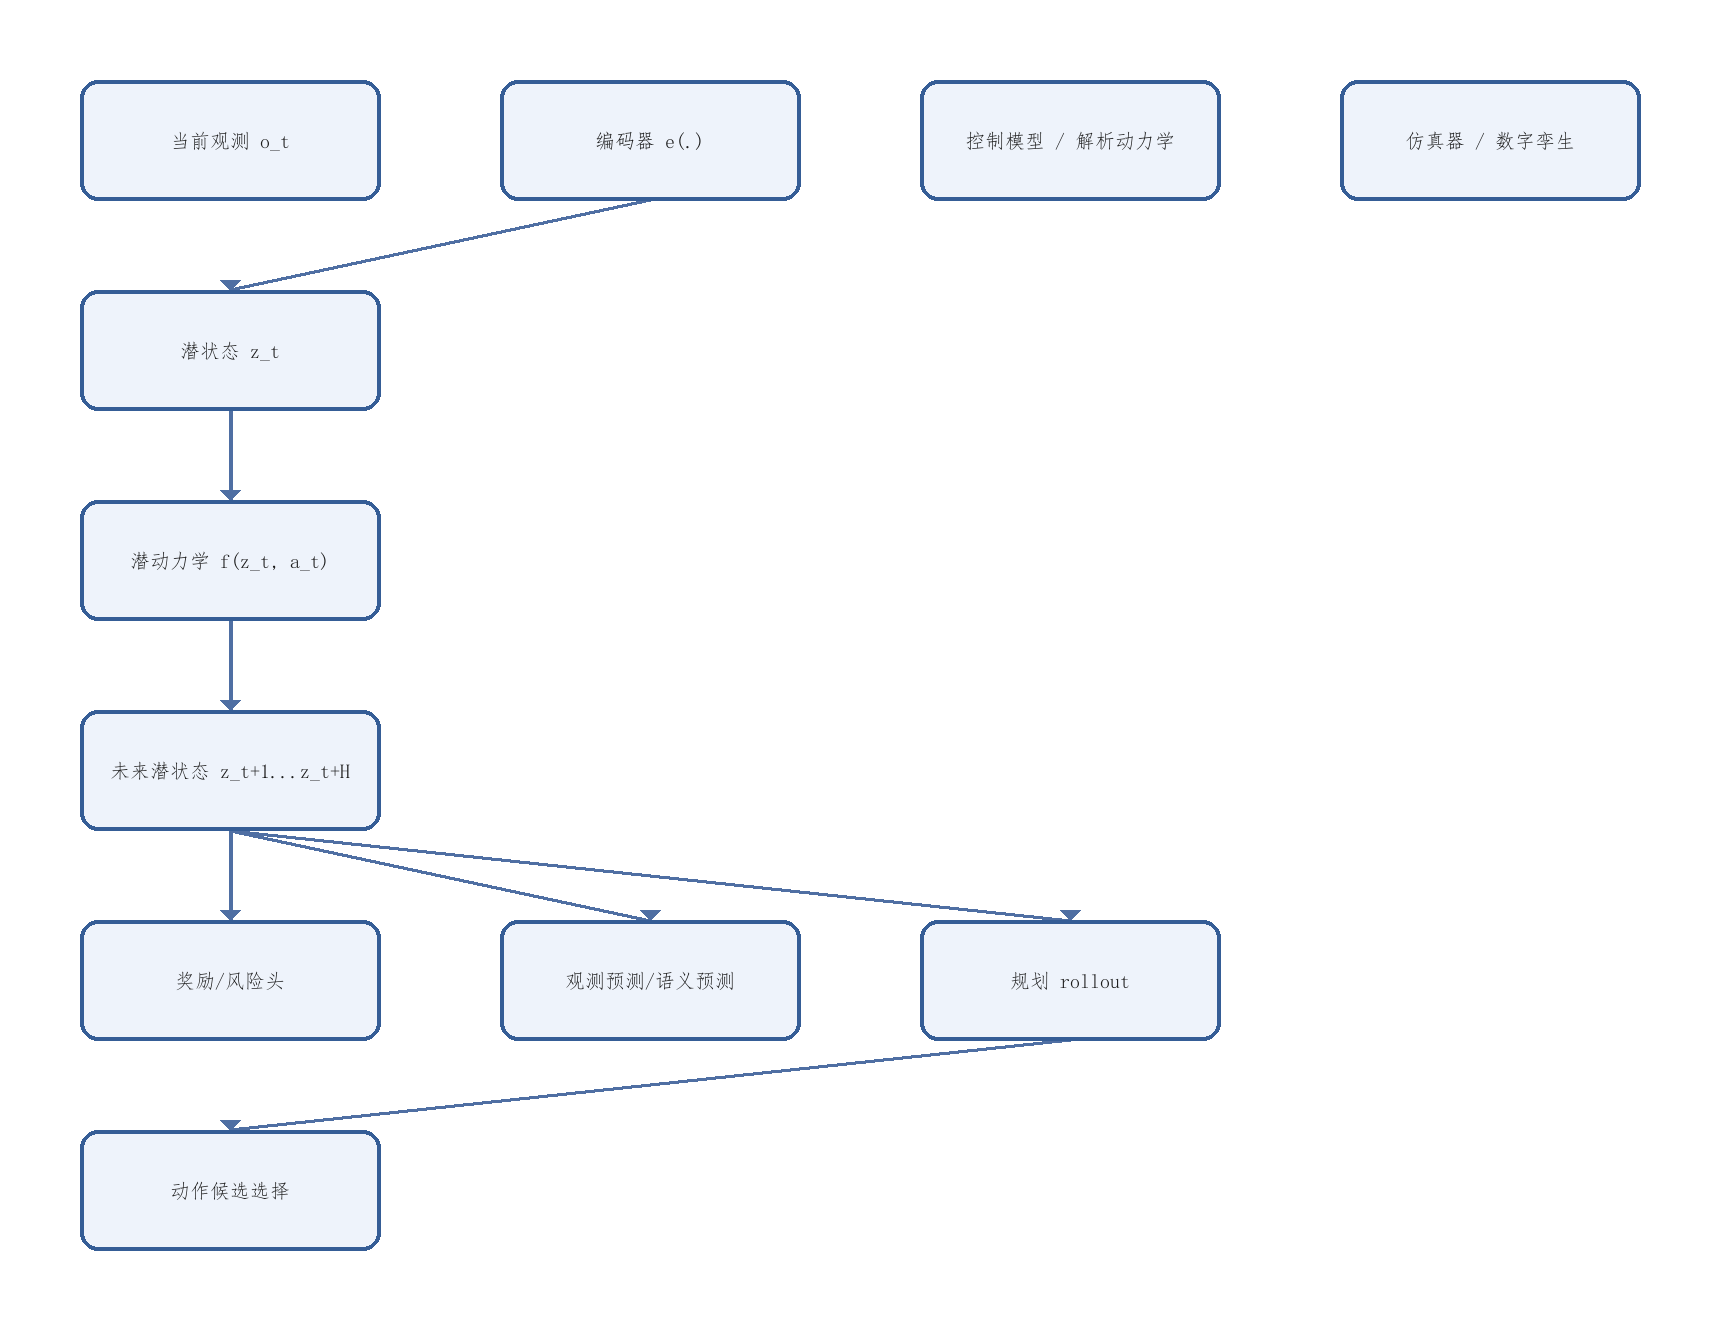
\includegraphics[width=0.9\textwidth,height=0.72\textheight,keepaspectratio]{figures/10-世界模型关系图.png}
\caption{10-世界模型关系图}
\label{fig:10-世界模型关系图}
\end{figure}
